\NewScheme{\SPOR}{SPOR}

\subsection{Message Passing through Predictive Onion Routes (PORs)}
\label{sec:message_passing}

\NewAlgorithm{\Send}{Send}
\NewAlgorithm{\Fwd}{Forward}
\NewAlgorithm{\Recv}{Receive}
\NewVariable{\rdv}{rdv}

In contrast to Tor~\cite{Tor} that provides only one address per hop
in the route, \name provides for each layer of the onion several
alternatives for the next hop in the route depending on their
probability of being online. We call our modified onion routes
Probabilistic Onion Routes or PORs.

Another difference from Tor, where connections are established by all
nodes in the route, \name is stateless. The sender
Alice and receiver Bob cooperate to create the headers containing all
the necessary routing information for future communication between
Alice and Bob. In that regard, we use two PORs: one to route packets from Alice to
Bob, and one for packets acknowledgement from Bob to Alice (See
Fig.~\ref{fig:file-exchange}~\ding{184}). We defined some fixed
parameters such as $L$, the number of layers in a POR, and
$\theta$, the stopping criterion for the layers creation, i.e the
maximum authorized  probability that all devices in a layer fail at
once.

To implement our  probabilistic
predictive onion routing mechanism, \name defined two different algorithms to
receive, send messages among users' \squad. For instance,
if Alice wants to send a message \(m\) to Bob, Bob uses the
\([Recv]\) algorithm (See \cref{SPORFwd}) to create a probabilistic onion route \(H_{Bob}\) from
 a set of rendez-vous point to its own devices from its \squad --- all the hops on the route are 
chosen by Bob uniformly at random from its RPS (\view).
 %\([Recv]\) returns the \(H_{Bob}\).
PORs have \(L\) layers, and for each layer the number of
alternatives nodes depends of a failure threshold \(\theta\). 
As long as \(\theta\) is not exceeded, alternatives nodes are added in
\(H_{Bob}\) as depicted in \cref{ExtendRoute}. Thus the probability of
failure for the extension is \(1 - (1 - \theta)^L\). In a similar
manner, Alice create an onion route \(H_{Alice}\) to enable Bob to
acknowledge its messages. Bob and Alice exchange then their calculated
PORs (i.e. H_{Bob} and H_{Alice}), using an
out-of-band channel, \eg using one device of their \squad (See
Fig.~\ref{fig:file-exchange}~\ding{182}).

\NewAlgorithm{\Store}{Store}

Once Alice get the \(H_{Bob}\), Alice uses \([Send]\) at some
later time to send the message to Bob using any of her devices from
its \squad (See \cref{SPORFwd}). First, \([Send]\) extends the route
\(H_{Bob}\) with some hops of Alice's choosing (uniformly randomly
chosen). Second, \([Send]\) extracts from the onion the first
layer, which contained the overall
possible alternative nodes $D$.
One device from $D$ is randomly chosen, and the \([Fwd]\)
sub-function is called as long as the message forwarding to one node of
the next layer is not successful (See \cref{SPORFwd}). Along the path, each node decrypts
in sequence the different layer with the current node’s private key. 
The end of the route is reached when the special value \(H_{Bob} = \top\) is
encountered. Consequently the ciphered message \(c_m\) is then stored
in the disk of the local node through the \([Store]\) sub function 
(\cref{SPORFwd}).

In a way similar, once Bob get the \(H_{Alice}\), Bob uses \([Send]\) at some
later time to acknowledge messages sent by Alice using any of his devices from
its\squad.

%The special value \(H = \top\) indicated the end of the route, thus \(c_m\) 
%    is intended for the local node and \(c_m\) is instead sent to disk using 
%    \(\Store\) (\cref{SPORFwd}).% 


%The SPOR.Forward algorithm forwards m down the route H, obtained by
%decrypting CH with the node’s associated private key. The special
%value H = ⊤ indicated the end of the route, thus cm is intended for
%the local node and cm is instead sent to disk using Store

%extends the route \(H_\rdv\) (using 
 %   \(\ExtendRoute\), \cref{ExtendRoute}) and sends the message \(m\) down the 
  %  extended route using the \(\SPOR[\Fwd]\) algorithm (\cref{SPORFwd}).
   % The first node of \(H_\rdv\) is the rendez-vous point selected by the 
    %recipient.

%It creates a probabilistic onion-route from a rendez-vous point to its own 
%    devices and returns the route to the sender.
 

\begin{figure}[t]
\center
  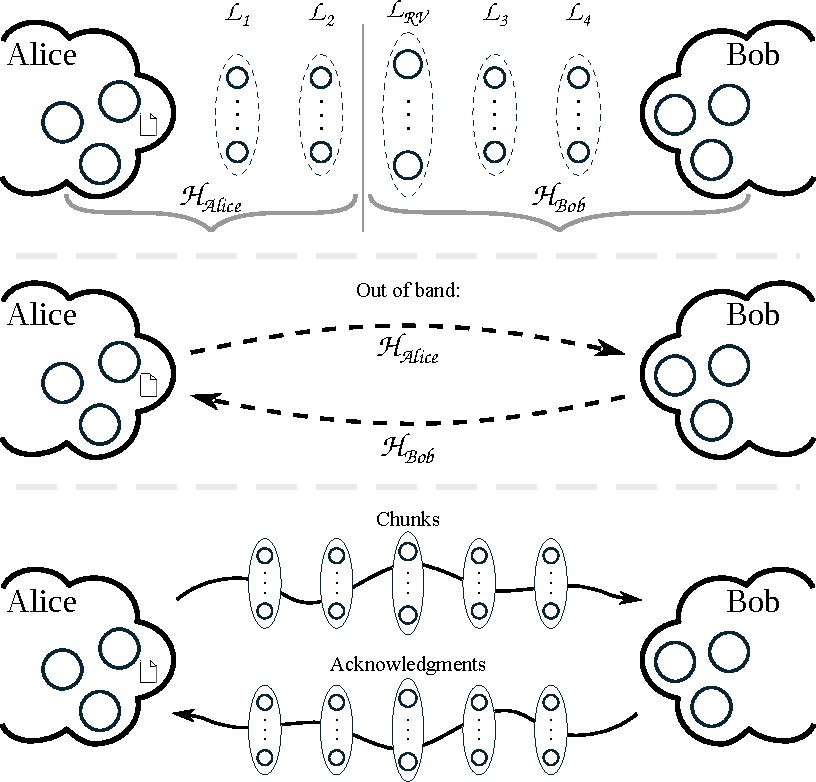
\includegraphics[scale=.55]{figures/file_exchange_v2.pdf}
  \caption{\label{fig:file-exchange}A schematic of the creation and usage of PORs between Alice and Bob's e-squads.}
\end{figure}

\NewAlgorithm{\ExtendRoute}{ExtendRoute}
\NewAlgorithm{\CreateOnionLayer}{CreateOnionLayer}


\begin{figure}
\framebox{\begin{minipage}{0.96\linewidth}
  \begin{algorithmic}[1]
\scriptsize
    \Function{\ExtendRoute}{$H, L$}
      \If{$L\leq 0$}
        \State \Return $H$
      \EndIf
      \State $D\gets \CreateOnionLayer[]$
      \State $H\gets D\concat \DeBEenc[\mpk, D, H]$
      \State \Return $\ExtendRoute[H, L-1, \theta]$
    \EndFunction
  \vspace{0.3em}
    \Function{\CreateOnionLayer}{}
      \State $(d, \pk_d, p_d)\gets \GetRandomPeer$
      \State $D\gets \{(d, \pk_d, p_d)\}$
      \While{$\prod_{d\in D} p_d > \theta$}
        \State $(d, \pk_d, p_d)\gets \GetRandomPeer$
        \State $D\gets D\cup \{(d, \pk_d, p_d)\}$
      \EndWhile
      \State \Return $D$
    \EndFunction
  \end{algorithmic}
  \end{minipage}}
  \caption{\label{ExtendRoute}%
    \scriptsize
    The \(\ExtendRoute\) algorithm extends a route \(H\)
  }
\end{figure}


\NewAlgorithm{\Dec}{Dec}
\NewVariable{\sk}{sk}

\begin{figure}
  \framebox{\begin{minipage}{0.96\linewidth}
  \begin{algorithmic}
\scriptsize
    \Require{%
      $D$ is the set of alternative recipient devices.
    }
    \Function{\Recv}{$D$}
      \State $H_\rdv\gets \ExtendRoute[D\concat \top, L, \theta]$
      \State \Return $H_\rdv$
        \Comment{Give to sender out-of-bound.}
    \EndFunction
  \end{algorithmic}
  %\end{minipage}}
%   \caption{\label{SPORFwd}%
% \scriptsize
%     The \(\Recv\) algorithm prepares the recipient for receiving a file.
%   }
  %\framebox{\begin{minipage}{0.96\linewidth}
  \begin{algorithmic}
\scriptsize
    \Require{%
      $m$ is the message to be sent,
      $H$ is the onion-route given by the recipient.
    }
    \Function{\Send}{$H,m$}
      \State $H\gets \ExtendRoute[H, L, \theta]$
      \State $D\concat C_H\gets H_\rdv$
      \For{$d\in D$}
        \Comment{Uniformly randomly chosen}
        \If{$d\method \Fwd[C_H, m] \neq \bot$}
          \State \Return $\top$
        \EndIf
      \EndFor
      \State \Return $\bot$
    \EndFunction
  \end{algorithmic}
  %\end{minipage}}
  % \caption{\label{SPORFwd}%
  %   \scriptsize
  %   The \(\Recv\), \(\Send\) and \(\Fwd\) algorithms.
  % }
 % \framebox{\begin{minipage}{0.96\linewidth}
  \begin{algorithmic}
\scriptsize
    \Require{$\sk$ is the private key-pair of the current node.}
    \Function{\Fwd}{$C_H, m$}
      \State $H\gets \DeBEdec[\mpk, \sk, C_H]$
      \If{$H = \bot$}
        \State \Return $\bot$
      \EndIf
      \State $\{d_i\}\concat C_H'\gets H$
      \If{$C_H' = \top$}
        \State \Return $\Store[m]$
      \EndIf
      \For{$d\in \{d_i\}$}
        \Comment{Uniformly randomly chosen}
        \If{$d\method \Fwd[C_H', m] \neq \bot$}
          \State \Return $\top$
        \EndIf
      \EndFor
      \State \Return $\bot$
    \EndFunction
    \Function{\Store}{$m$}
      \State $m\gets \DeBEdec[\mpk, \sk, c_m]$
      \If{$m = \bot$}
        \State \Return $\bot$
      \EndIf
      \State Store $m$ to disk.
      \State \Return $\top$
    \EndFunction
  \end{algorithmic}
  \end{minipage}}
  \caption{\label{SPORFwd}%
    \scriptsize
    The \(\Recv\) (prepares the recipient for receiving a file), \(\Send\) and \(\Fwd\) (forwards \(m\) down the route \(H\)) algorithms.
  }
\end{figure}

